\cohead{\Large\textbf{Änderungsraten}}
\fakesubsection{Änderungsraten}
Oft ist der Wert einer Größe von einer anderen Größe abhängig, z.B. ändert sich die Geschwindigkeit eines Autos in Abhängigkeit der Zeit oder die Temperatur ändert sich in Abhängigkeit der Zeit. In der Realität sind die meisten Größen von mehreren Variablen abhängig, so ändert sich die Temperatur nicht nur mit der Zeit, sondern auch mit dem Ort (der selbst wieder dreidimensional ist und somit von drei Größen abhängt). Wir werden uns auf Fälle beschränken, in denen die betrachtete Größe von genau einer anderen Größe abhängt.
\begin{tcolorbox}
	\phantom{ }\\
	\textcolor{loestc}{Die Änderungsrate einer Größe bezüglich einer Variablen gibt an, wie stark sich die Größe ändert, wenn man den Wert der Variablen ändert.}\\
\end{tcolorbox}
In den meisten Beispielen aus dem Alltag betrachtet man die Änderung einer Größe über die Zeit. Betrachten wir als Beispiel den Kurs des DAX:\\
\begin{minipage}[t]{\textwidth}
	\centering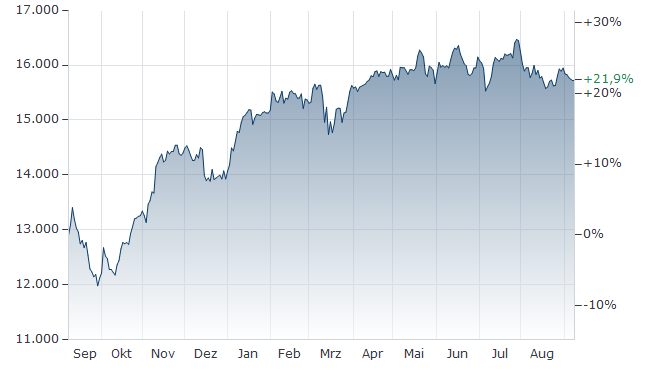
\includegraphics{\ableitung/pics/chart.png}
\end{minipage}\\
Von Anfang Oktober bis Ende Dezember ist der Kurs von ca. 12.250 Punkten auf ca 14.100 Punkte erhöht. Der Unterschied innerhalb von 3 Monaten beträgt also 1850 Punkte. Die durchschnittliche Änderungsrate oder auch mittlere Änderungsrate entspricht dann \(\frac{1850\text{ Punkte}}{3\text{ Monate}}\approx 617\frac{\text{Punkte}}{\text{Monat}}\). Im Mittel ist der DAX also von Anfang Oktober bis Ende Dezember um 617 Punkte pro Monat gestiegen. Würden wir die Achsen des Charts wie üblich mit x-Achse und y-Achse bezeichnen, so lässt sich die mittlere Änderungsrate berechnen, indem man den Unterschied der y-Werte durch den Unterschied der x-Werte teilt.\newpage
Die mittlere oder durchschnittliche Änderungsrate einer Funktion \(f(x)\) auf dem Intervall \([x_1,\ x_2]\) lässt sich allgemein wie folgt bestimmen:
\begin{tcolorbox}
	\textbf{Mittlere Änderungsrate}\\
	\Large$\makebox[\linewidth]{\textcolor{loestc}{\(\dfrac{f(x_2)-f(x_1)}{x_2-x_1}\)}}$
\end{tcolorbox}
Diesen Ausdruck kennen wir bereits. Sind von einer Geraden zwei Punkte \(P_1(x_1\vert f(x_1))\) und \(P_2(x_2\vert f(x_2))\) gegeben, so bestimmt der obige Ausdruck die Steigung der Geraden. Tatsächlich kann man die mittlere Änderungsrate als durchschnittliche Steigung der Funktion auffassen. Betrachten wir als Beispiel \(f(x)=x^2\):\\
\begin{minipage}{\textwidth}
	\begin{minipage}{0.49\textwidth}
		\centering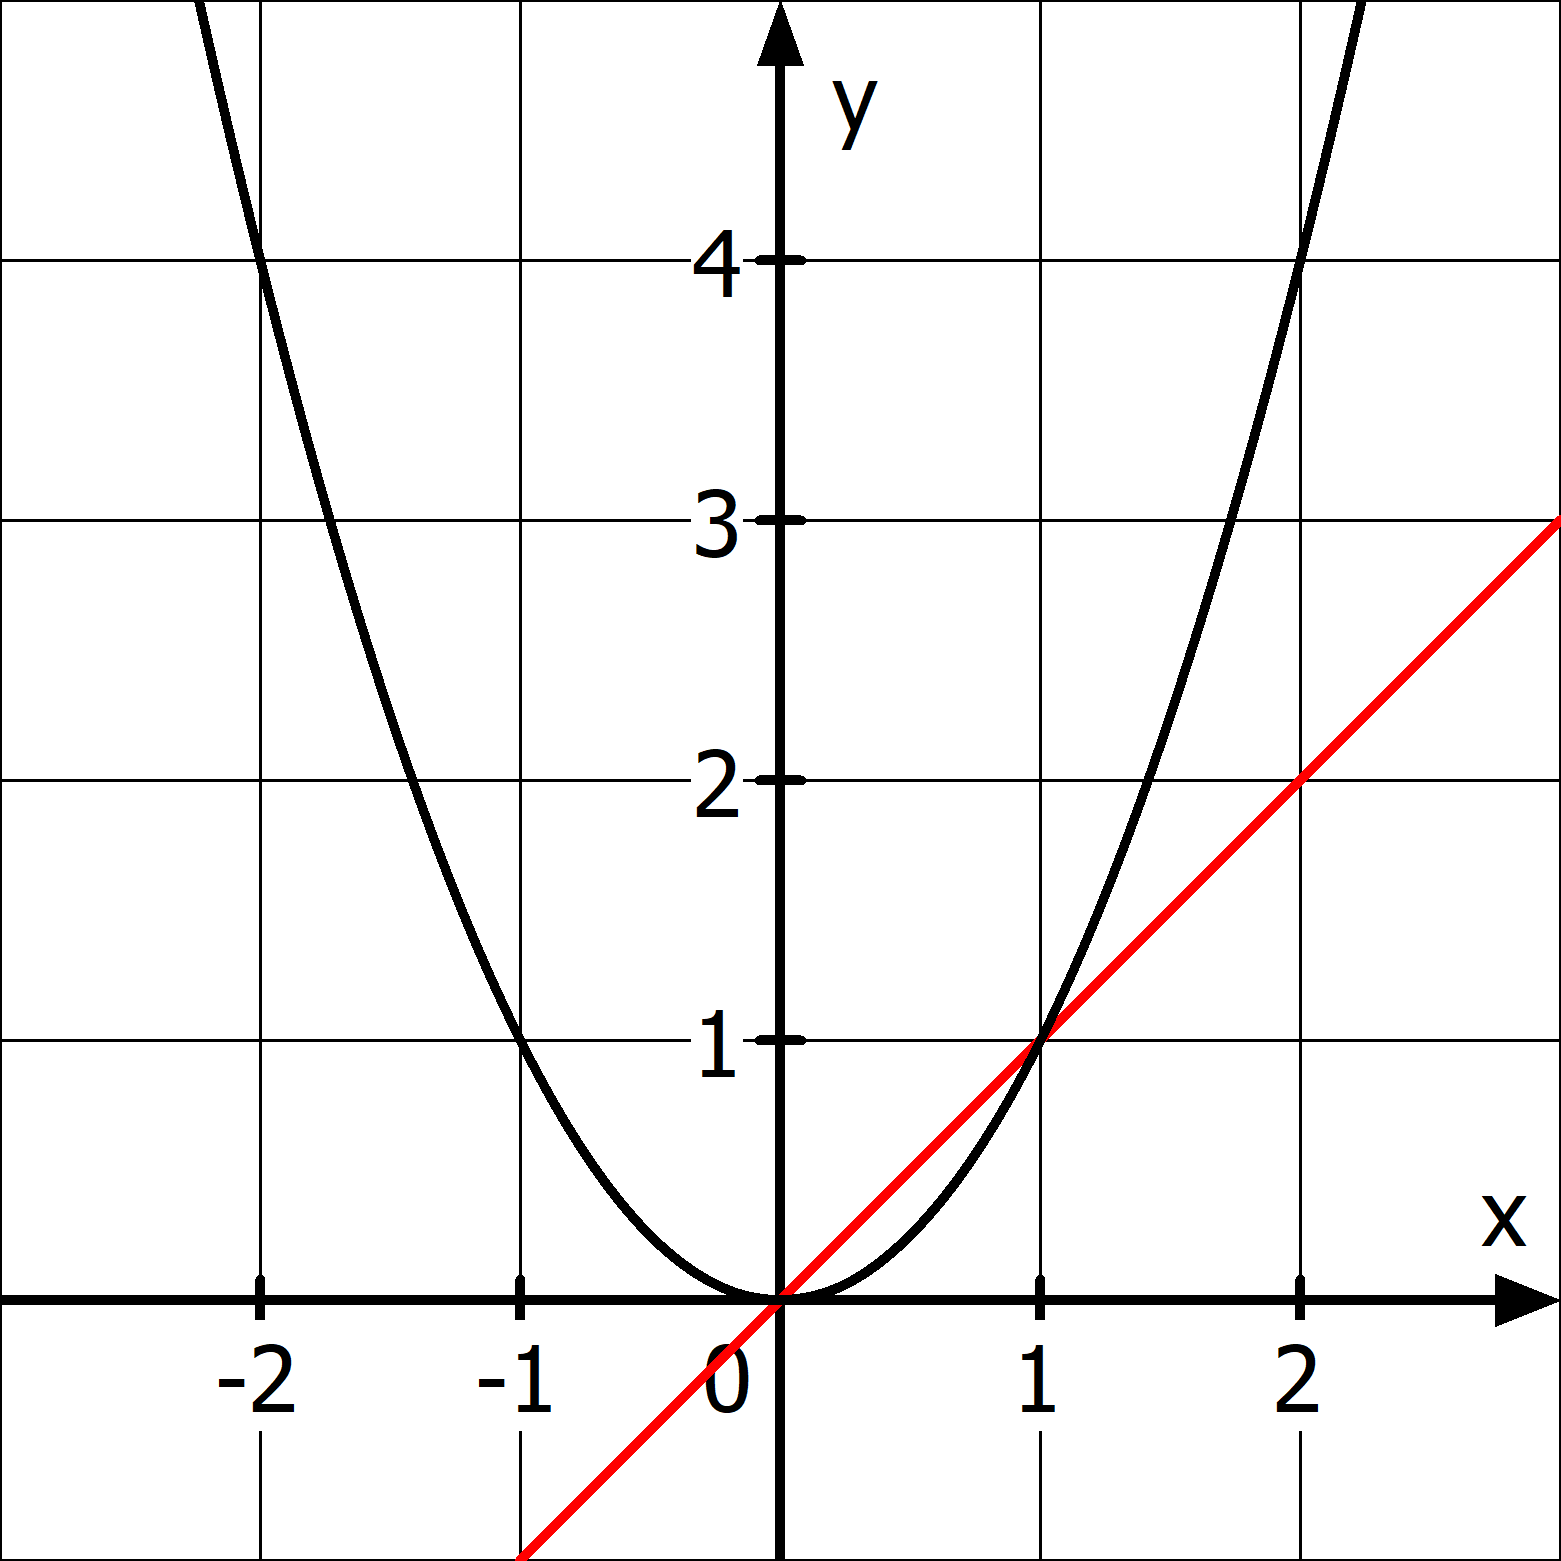
\includegraphics[width=.95\textwidth]{\ableitung/pics/mittAenderungsrate.png}
	\end{minipage}
	\begin{minipage}{0.49\textwidth}
		Die mittlere Änderungsrate im Intervall \(\textcolor{red}{[0,\ 1]}\) entspricht dann der Steigung der Geraden durch die Punkte \(\textcolor{red}{P_1(0\vert f(0)=0)}\) und \(\textcolor{red}{P_2(1\vert f(1)=1)}\): \(\textcolor{red}{\frac{1-0}{1-0}=1}\).\\
		Die mittlere Änderungsrate im Intervall \(\textcolor{blue}{[0,\ 2]}\) entspricht:\\
		\(\textcolor{loes}{\frac{4-0}{2-0}=2}\)\vspace{0.5cm}\\
		Die mittlere Änderungsrate im Intervall \(\textcolor{ForestGreen}{[-2,\ -1]}\) entspricht:\\
		\(\textcolor{loes}{\frac{1-4}{-1-(-2)}=-3}\)\vspace{1cm}
	\end{minipage}
\end{minipage}\vspace{.5cm}
Die mittlere Änderungsrate einer Funktion auf einem Intervall gibt also an, wie weit man im Schnitt nach oben (positive Änderungsrate) oder nach unten (negative Änderungsrate) gehen muss, wenn man einen Schritt nach rechts macht, um vom linken Punkt auf den rechten Punkt zu kommen. Wie die Funktion vor dem Intervall, im Intervall und nach dem Intervall verläuft, spielt für die mittlere Änderungsrate keine Rolle. Es kommt nur auf den Funktionswert am Beginn des Intervalls und am Endes des Intervalls an.\\
Beispielsweise haben die Funktionen \(g(x)=0,75x^2\) und \(h(x)=e^{\ln(2)x}\) auf dem Intervall \([0,\ 2]\) die gleiche mittlere Änderungsrate:\\
Mittlere Änderungsrate von \(g(x)\): \(\dfrac{g(2)-g(0)}{2-0}=\frac{3}{2}=1,5\)\\
Mittlere Änderungsrate von \(h(x)\): \(\dfrac{h(2)-h(0)}{2-0}=\frac{4-1}{2}=1,5\)
\newpage
%%%%%%%%%%%%%%%%%%%%%%%%%%%%%%%%%%%%%%%%%%%%%%%%%%%%%%%%%%%%%%%%%%%%%%%%%%%%%%%%%%%%%%%%%%%%%%%%%%%%%%
\begin{minipage}{\textwidth}
	\begin{Exercise}[title={Bestimme die durchschnittliche Änderungsrate des DAX für folgende Zeiträume jeweils pro Monat.}, label=aenderungsrateA1]
		\begin{enumerate}[label=\alph*)]
			\item Von Anfang Oktober bis Ende Februar.
			\item Von Anfang Oktober bis Ende Juli.
			\item Von Anfang Januar bis Ende Mai.
			\item Von Anfang Dezember bis Ende Dezember.
		\end{enumerate}
	\end{Exercise}
\end{minipage}
\begin{minipage}{\textwidth}
	\begin{Exercise}[title={Bestimme jeweils die durchschnittliche Änderungsrate auf den Intervallen \(I_1=[0,\ 2]\) sowie \(I_2=[-2,\ 2]\) und \(I_3=[-1,\ 4]\). Du kannst auf 2 Nachkommastellen runden, falls notwendig.}, label=aenderungsrateA2]
		\begin{enumerate}[label=\alph*)]
			\item \(f_1(x)=3x\)
			\item \(f_2(x)=-2x^2\)
			\item \(f_3(x)=x^3-2x^2\)
			\item \(f_4(x)=e^x\)
			\item \(f_5(x)=2e^{3x}-4\)
			\item \(f_6(x)=-0,1x^3\)
			\item \(f_7(x)=x+10\)
			\item \(f_8(x)=-e^x+x-2\)
			\item \(f_9(x)=-\frac{3}{4}x^2+3x\)
		\end{enumerate}
	\end{Exercise}
\end{minipage}
%%%%%%%%%%%%%%%%%%%%%%%%%%%%%%%%%%%%%%%%%
\begin{Answer}[ref=aenderungsrateA1]
	\begin{enumerate}[label=\alph*)]
		\item Von Anfang Oktober bis Ende Februar.\\
		\(\frac{15.200\text{ Punkte}-12.250\text{ Punkte}}{5\text{ Monate}}= 590\frac{\text{Punkte}}{\text{Monat}}\)
		\item Von Anfang Oktober bis Ende Juli.\\
		\(\frac{16.100\text{ Punkte}-12.250\text{ Punkte}}{10\text{ Monate}}= 385\frac{\text{Punkte}}{\text{Monat}}\)
		\item Von Anfang Januar bis Ende Mai.\\
		\(\frac{15.750\text{ Punkte}-14.000\text{ Punkte}}{5\text{ Monate}}= 350\frac{\text{Punkte}}{\text{Monat}}\)
		\item Von Anfang Dezember bis Ende Dezember.\\
		\(\frac{14.000\text{ Punkte}-14.400\text{ Punkte}}{1\text{ Monat}}=-400\frac{\text{Punkte}}{\text{Monat}}\)\\
		Die mittlere Änderungsrate ist negativ, da der Kurs gefallen ist.
	\end{enumerate}
\end{Answer}
\begin{Answer}[ref=aenderungsrateA2]
	\begin{enumerate}[label=\alph*)]
		\item \(f_1(x)=3x\)\\
		mittlere Änderungsrate auf \(I_1=[0,\ 2]\): \(\frac{6-0}{2-0}=3\)\\
		mittlere Änderungsrate auf \(I_2=[-2,\ 2]\): \(\frac{6-(-6)}{2-(-2)}=3\)\\
		mittlere Änderungsrate auf \(I_3=[-1,\ 4]\): \(\frac{12-(-3)}{4-(-1)}=3\)\\
		Anmerkung: Da es sich um eine Gerade handelt, ist die mittlere Änderungsrate immer gleich der Steigung der Geraden.
		\item \(f_2(x)=-2x^2\)\\
		mittlere Änderungsrate auf \(I_1=[0,\ 2]\): \(\frac{-8-0}{2-0}=-4\)\\
		mittlere Änderungsrate auf \(I_2=[-2,\ 2]\): \(\frac{-8-(-8)}{2-(-2)}=0\)\\
		mittlere Änderungsrate auf \(I_3=[-1,\ 4]\): \(\frac{-32-(-2)}{4-(-1)}=-6\)\\
		\item \(f_3(x)=x^3-2x^2\)\\
		mittlere Änderungsrate auf \(I_1=[0,\ 2]\): \(\frac{0-0}{2-0}=0\)\\
		mittlere Änderungsrate auf \(I_2=[-2,\ 2]\): \(\frac{0-(-16)}{2-(-2)}=4\)\\
		mittlere Änderungsrate auf \(I_3=[-1,\ 4]\): \(\frac{32-(-3)}{4-(-1)}=7\)\\
		\item \(f_4(x)=e^x\)\\
		mittlere Änderungsrate auf \(I_1=[0,\ 2]\): \(\frac{7,39-1}{2-0}=3,19\)\\
		mittlere Änderungsrate auf \(I_2=[-2,\ 2]\): \(\frac{7,39-0,14}{2-(-2)}=1,81\)\\
		mittlere Änderungsrate auf \(I_3=[-1,\ 4]\): \(\frac{54,60-0,37}{4-(-1)}=10,85\)\\
		\item \(f_5(x)=2e^{3x}-4\)\\
		mittlere Änderungsrate auf \(I_1=[0,\ 2]\): \(\frac{802,86-(-2)}{2-0}=402,43\)\\
		mittlere Änderungsrate auf \(I_2=[-2,\ 2]\): \(\frac{802,86-(-4,00)}{2-(-2)}=201,71\)\\
		mittlere Änderungsrate auf \(I_3=[-1,\ 4]\): \(\frac{325.505,58-(-3,90)}{4-(-1)}=65.101,90\)\\
		\item \(f_6(x)=-0,1x^3\)\\
		mittlere Änderungsrate auf \(I_1=[0,\ 2]\): \(\frac{-0,8-0}{2-0}=-0,4\)\\
		mittlere Änderungsrate auf \(I_2=[-2,\ 2]\): \(\frac{-0,8-0,8}{2-(-2)}=-0,4\)\\
		mittlere Änderungsrate auf \(I_3=[-1,\ 4]\): \(\frac{-6,4-0,1}{4-(-1)}=-1,3\)\\
		\item \(f_7(x)=x+10\)\\
		mittlere Änderungsrate auf \(I_1=[0,\ 2]\): \(\frac{12-10}{2-0}=1\)\\
		mittlere Änderungsrate auf \(I_2=[-2,\ 2]\): \(\frac{12-8}{2-(-2)}=1\)\\
		mittlere Änderungsrate auf \(I_3=[-1,\ 4]\): \(\frac{14-9}{4-(-1)}=1\)\\
		Auch hier hätte man die mittleren Änderungsraten direkt aus der Steigung bestimmen können.
		\item \(f_8(x)=-e^x+x-2\)\\
		mittlere Änderungsrate auf \(I_1=[0,\ 2]\): \(\frac{-7,39-(-3)}{2-0}=-2,19\)\\
		mittlere Änderungsrate auf \(I_2=[-2,\ 2]\): \(\frac{-7,39-(-4,14)}{2-(-2)}=-0,81\)\\
		mittlere Änderungsrate auf \(I_3=[-1,\ 4]\): \(\frac{-52,60-(-3,37)}{4-(-1)}=-9,85\)\\
		\item \(f_9(x)=-\frac{3}{4}x^2+3x\)\\
		mittlere Änderungsrate auf \(I_1=[0,\ 2]\): \(\frac{3-0}{2-0}=1,5\)\\
		mittlere Änderungsrate auf \(I_2=[-2,\ 2]\): \(\frac{3-(-9)}{2-(-2)}=3\)\\
		mittlere Änderungsrate auf \(I_3=[-1,\ 4]\): \(\frac{0-(-3,75)}{4-(-1)}=0,75\)\\
	\end{enumerate}
\end{Answer}